\documentclass[12pt, a4paper, oneside]{ctexart}
\usepackage{amsmath, amsthm, amssymb, bm, color, framed, graphicx, hyperref, mathrsfs, mathtools, enumerate, tikz}
\usepackage{graphicx}
\usepackage{float}
\usepackage{subfig}

\usetikzlibrary{patterns}

\title{\textbf{Homework 3}}
\author{萃英学院\qquad 2022级\qquad 王一鑫}
\date{\today}
\linespread{1.5}
\newcounter{problemname}
\newenvironment{problem}{\begin{framed}\stepcounter{problemname}\par\noindent\textsc{Problem \arabic{problemname}. }}{\end{framed}\par}
\newenvironment{solution}{%
	\par\noindent\textsc{Solution. }\ignorespaces
}{%
	\hfill$\qed$\par
}
\newenvironment{note}{\par\noindent\textsc{Note of Problem \arabic{problemname}. }}{\\\par}

\begin{document}
	
	\maketitle
	
	\begin{problem}
		(Exercise 2.18)
		
		\begin{enumerate}[(a)]
			\item A connected graph is Eulerian if and only if its set of edges can be split up into edge-disjoint cycles
			
			\item A connected graph is semi-Eulerian if and only if it has exactly two vertices of odd degree.
		\end{enumerate}
	\end{problem}
	
	\begin{solution}
		\begin{enumerate}[(a)]
			\item  We prove by induction on the number of edges.  Assume $G$ has $n > 0$ (since the case $n = 0$ is trivial) edges and the statement holds
			for all graphs with fewer than $n$ edges.

			If $G$ has more than one connected component, the claim holds for each (smaller) component,
			hence for all of $G$. Hence we now assume that $G$ is connected. 

			$\Rightarrow$: Consider an Eulerian trail $v_0 v_1 v_2 \dots v_n$ with $v_0 = v_n$. Consider all $(i, j)$ with $0 \leq i < j \leq n$ and
			$v_i = v_j$. Such pairs exist because $v_0 = v_n$ (and $n > 0$). Select $(i, j)$ among these pairs such that
			$j - i$ is minimized. Then $v_i v_{i+1} \dots v_j$ is a simple cycle $\gamma$ and $v_0 \dots v_i v_{j+1} \dots v_n$ is an Eulerian trail
			of the graph $G' := G - \gamma$. By induction, $G'$ can be split up into edge-disjoint cycles. Together with
			$\gamma$ we obtain a partitioning of $G$ into edge-disjoint cycles.

			$\Leftarrow$: Assume $G$ can be split up into edge-disjoint cycles. Since $n > 0$, there must be at least one cycle
			in this partitioning. If there is exactly one cycle, it is automatically an Eulerian trail and we are done.
			we remove from $G$ the edges of $C$ to form a new (possibly disconnected) graph $H$ with fewer edges than $G$, and H can also be split
			up into edge-disjoint cycles. By the induction hypothesis, each
			component of $H$ has an Eulerian trail. But each component of $H$ has at least one vertex in common with $C$, by connectedness. 
			
			It follows that we can obtain the required
			Eulerian trail of $G$ by tracing the edges of $C$ until a non-isolated vertex of $H$ is
			reached, tracing the Eulerian trail of the component of $H$ that contains that vertex, and
			then continuing along the edges of $C$ until we reach a vertex belonging to another
			component of $H$, and so on. The whole process terminates when we return to the
			initial vertex. See Figure \ref{fig:Schema}.

			\begin{figure}[H]
				\small
				\centering
				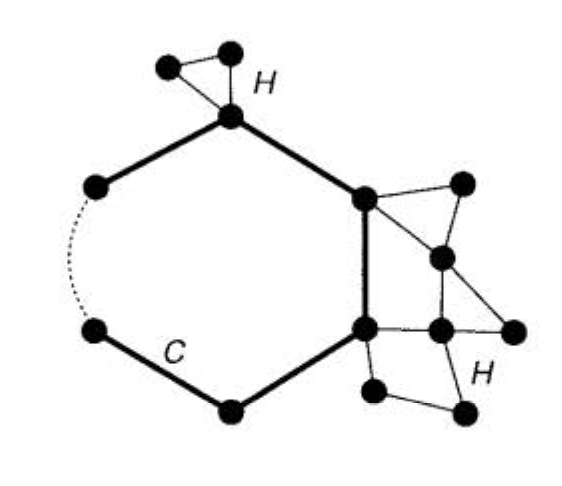
\includegraphics[width=0.45\columnwidth]{figure/fig3.png}
				\caption{Schema}
				\label{fig:Schema}
			\end{figure}

			\item $\Rightarrow$ Suppose that $P$ is a non-closed trail that includes every edge of $G$. Whenever $P$ passes through a vertex, there is a 
			contribution of $2$ towards the degree of that vertex, except the original and the end points. Since each edge 
			occurs exactly once in $P$, the degree of each vertex must be a sum of $2s$, except two vertices of odd degree.

			$\Leftarrow$: The proof is by induction on the number of edges of $G$. Suppose that $G$ has two vertices of odd degree.
			Since $G$ is connected, each vertex has degree at least $2$ and so $G$ contains a cycle $C$.

			we remove from $G$ the edges of $C$ to form a new (possibly disconnected) graph $H$ with fewer edges than $G$, and H has exactly two vertices of odd degree.
			By the induction hypothesis, H is semi-Eulerian, and each component of $H$ has at least one vertex in common with $C$, by connectedness. 
			
			It follows that we can obtain the required non-closed
			Eulerian trail of $G$ by starting from one of the vertex of odd degree, and tracing the edges of $H$ until a non-isolated vertex of $C$ is
			reached, tracing the edges of $C$ that incident with that vertex until we reach a vertex belonging to another component of $H$, and so on. Finally we end at another vertex of odd degree in H.
			
		\end{enumerate}
	\end{solution}
		

		
	
	\begin{problem}
		(Exercise 2.19)
		
		Let $G$ be a connected graph with $k(>0)$ vertices of odd degree.

		\begin{enumerate}[(i)]
			\item Show that the minimum number of trails, that have no edges in common, is $\frac{1}{2}k$.
			\item How many continuous pen-strokes are needed to draw the diagram in Fig\ref{fig:problem2} without repeating any line?
		\end{enumerate}
		
		\begin{figure}[H]
			\small
			\centering
			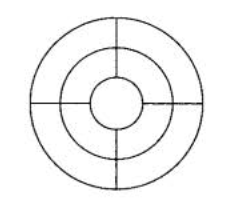
\includegraphics[width=0.25\columnwidth]{figure/fig1.png}
			\caption{Figure for problem 2}
			\label{fig:problem2}
		\end{figure}


	\end{problem}
	
	\begin{solution}
		\begin{enumerate}[(i)]
			\item At least $\dfrac{1}{2}k$ trails are needed, so as to use up all $k$ vertices of odd degree.
			
			If we now add $\dfrac{1}{2}k$ edges to $G$ and join these vertices in pairs, then we obtain an Eulerian graph $G^{\prime}$
			, since the degree of each vertex of $G^{\prime}$ is even.  We then  obtain the require $\dfrac{1}{2}k$ trails by writing down an Eulerian trail for $G^{\prime}$ and then omitting the added edges.
			\item Since the graph has $8$ vertices of odd degree, then there are at least $4$ trails which have no edges in common. That is, $4$ continuous pen-strokes are needed
			to draw the diagram.
		\end{enumerate}
		
	\end{solution}
	
	\begin{problem}
		(Exercise 2.21)
		
		An Eulerian graph is \textbf{randomly traceable} from a vertex $v$ if, whenever we start from $v$ and traverse the graph in an arbitrary way never using any edge twice, we eventually obtain an Eulerian trail.

		\begin{enumerate}[(i)]
			\item Show that the graph in Fig\ref{fig:problem3} is randomly traceable.
			\begin{figure}[H]
				\small
				\centering
				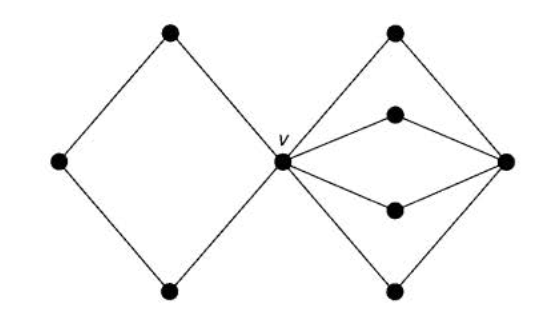
\includegraphics[width=0.5\columnwidth]{figure/fig2.png}
				\caption{Figure for problem 3}
				\label{fig:problem3}
			\end{figure}
			\item Give an example of an Eulerian graph that is not randomly traceable.
			\item Why might a randomly traceable graph be suitable for the layout of an exhibition.
		\end{enumerate}
		
	\end{problem}
	
	\begin{solution}
		
		\begin{enumerate}[(i)]
			\item The edges of $G$ can be split into three cycles in different ways, but all have the common vertex $v$. For example, ont of the partitioning is shown as Fig \ref{fig:partitioning}.
			\begin{figure}[H]
				\small
				\centering
				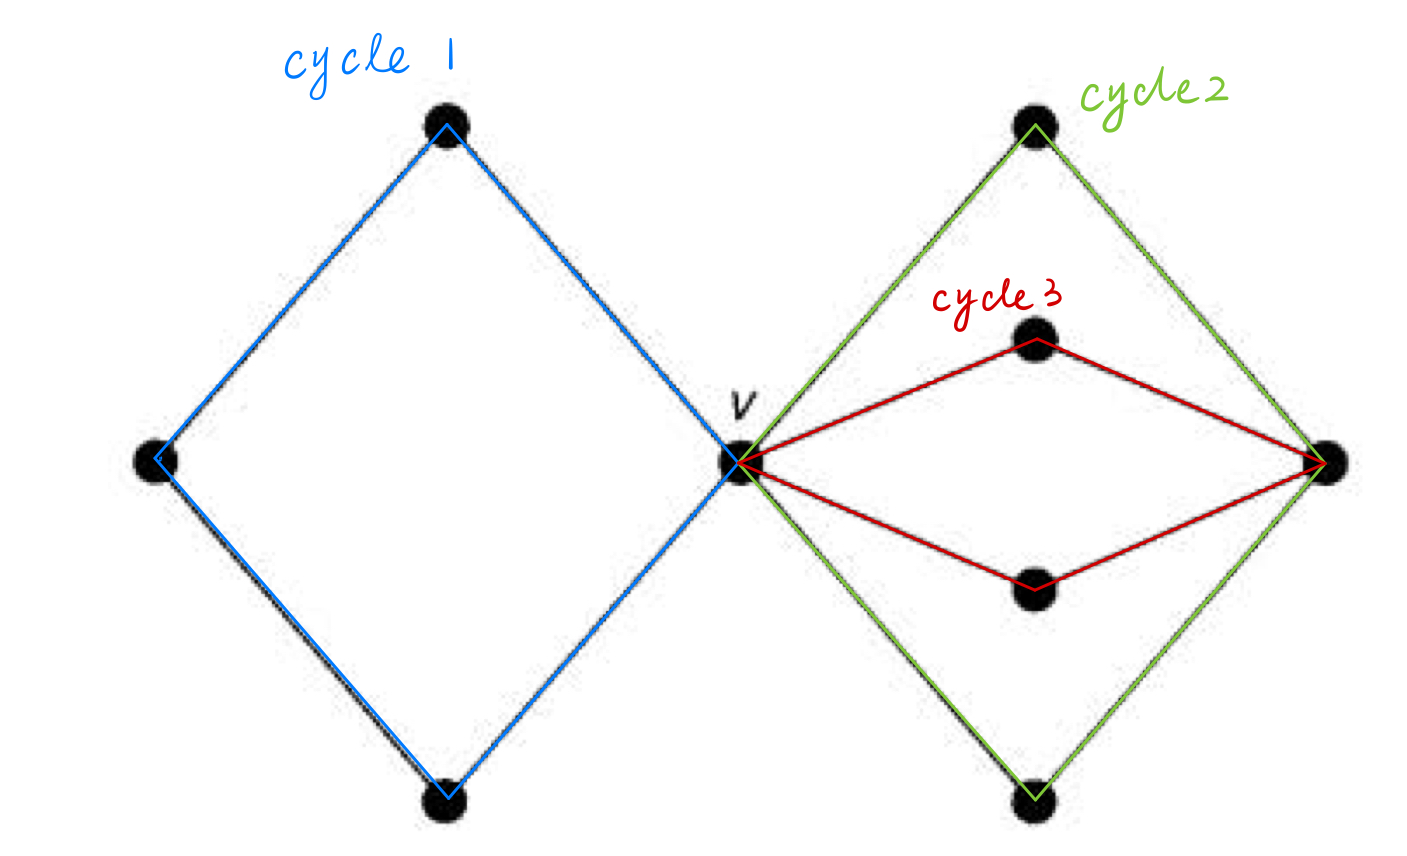
\includegraphics[width=0.5\columnwidth]{figure/fig4.png}
				\caption{Example of partitioning}
				\label{fig:partitioning}
			\end{figure}
			Starting from $v$ and traverse the graph in an arbitrary way will trace the three cycles seperately,
			and we eventually obtain an Eulerian trail never using any edge twice. Thus the graph is randomly traceable.

			\item Change the vertex $v$ to be the leftmost one. Shown as Fig \ref{fig:conterexample}.
			\begin{figure}[H]
				\small
				\centering
				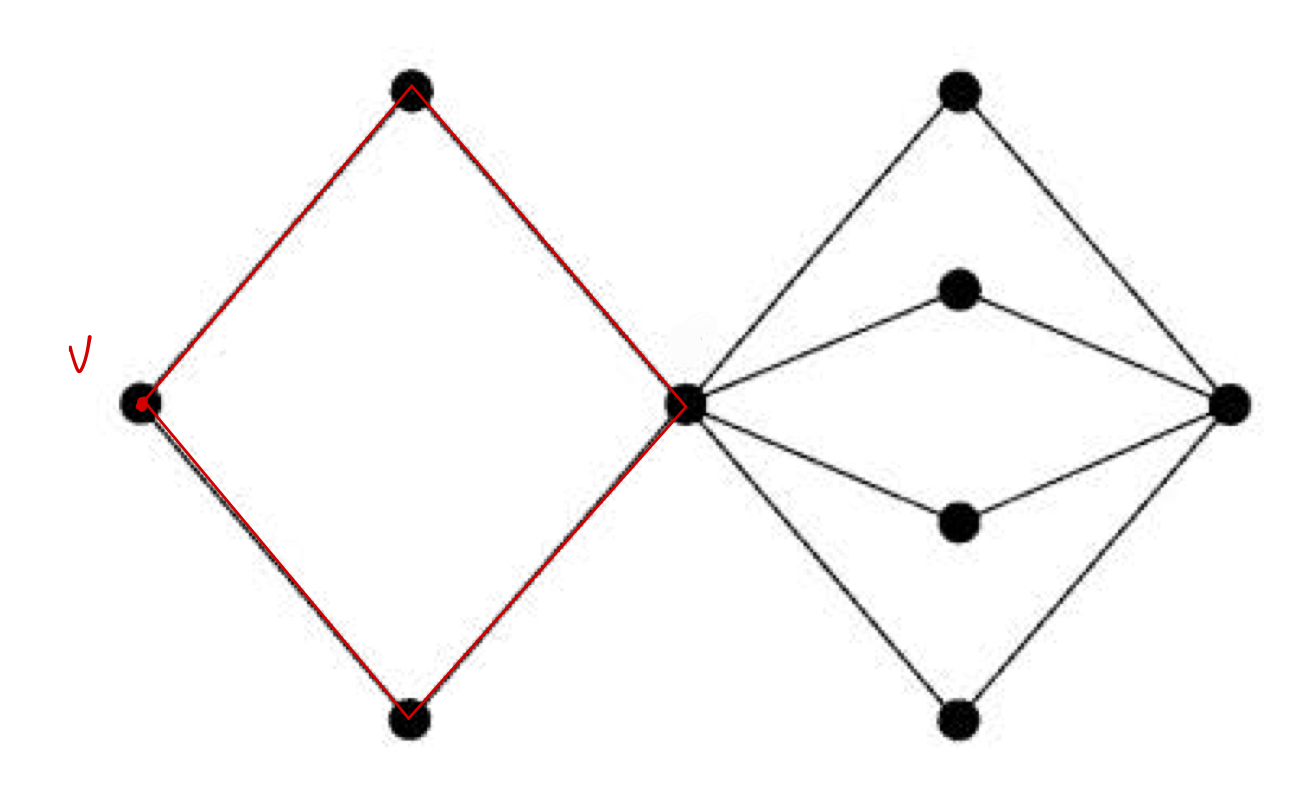
\includegraphics[width=0.5\columnwidth]{figure/fig5.png}
				\caption{conterexample}
				\label{fig:conterexample}
			\end{figure}

			\item A randomly traceable graph ensures that visitors can navigate the exhibition in any direction without retracing their steps, making sure they can enjoy the whole exhibition without going down the same way.
		\end{enumerate}
		
		
	\end{solution}
	
	
	
	\begin{problem}
		(Exercise 2.24)

		Let \( D \) be the digraph whose vertices are the pairs of integers \( 11, 12, 13, 21, 22, 23, 31, 32, 33 \), and whose arcs join \( ij \) to \( kl \) if and only if \( j = k \). Find an Eulerian trail in \( D \) and use it to obtain a circular arrangement of nine 1s, nine 2s, and nine 3s in which each of the 27 possible triples \( (111, 233, \dots) \) occurs exactly once. (Problems of this kind arise in communication theory.)
		
		
	\end{problem}
	
	\begin{solution}
		Actually, we can start from $11$ and finally return to $11$. Every vertex of $D$ has indegree
		and outdegree $3$, it may have many Euler trails. I found one of these Euler trails is
		\[\begin{aligned}
			&11 \to 12 \to 21 \to 12 \to 22 \to 22 \to 21 \to 11 \to 13 \to\\
			&33	\to 31 \to 13 \to 31 \to 12 \to 23 \to 33 \to 33 \to 32 \to\\
			&21 \to 13 \to 32 \to 23 \to 32 \to 22 \to 23 \to 31 \to 11 
		\end{aligned}\]	
		Then we can use it to obtain a  circular arrangement like 
		\[112122211331312333213232231\]
		Since it has $27$ digits, it has $27$ three-digit substrings, like the $212$ that starts at position $3$. 
		That substring arises from the edge going from vertex $21$ to vertex $12$; 
		we used that edge only once, so there can be only one $212$substring. 
		Thus, each of the $27$ possible three-digit substrings must be represented exactly once in our string.
	\end{solution}


	\begin{problem}
		(Exercise 2.26)

		\begin{enumerate}[(a)]
			\item Find an Eulerian trail in the infinite triangular lattice $S$.
			\item Verify that $S$ satisfies the conditions of Theorem 2.14. i.e., $G$ is a 
			countable connected graph which is Eulerian.
				
		\end{enumerate}
		
		
	\end{problem}
	
	\begin{solution}
		\begin{enumerate}
			\item We draw the Eulerian trail in the infinite triangular lattice $S$ by the following figures.

		The number in the edge shows the order we connect the lines.
		\begin{figure}[h]
	
			\begin{minipage}{0.32\linewidth}
				\vspace{3pt}
				
				\centerline{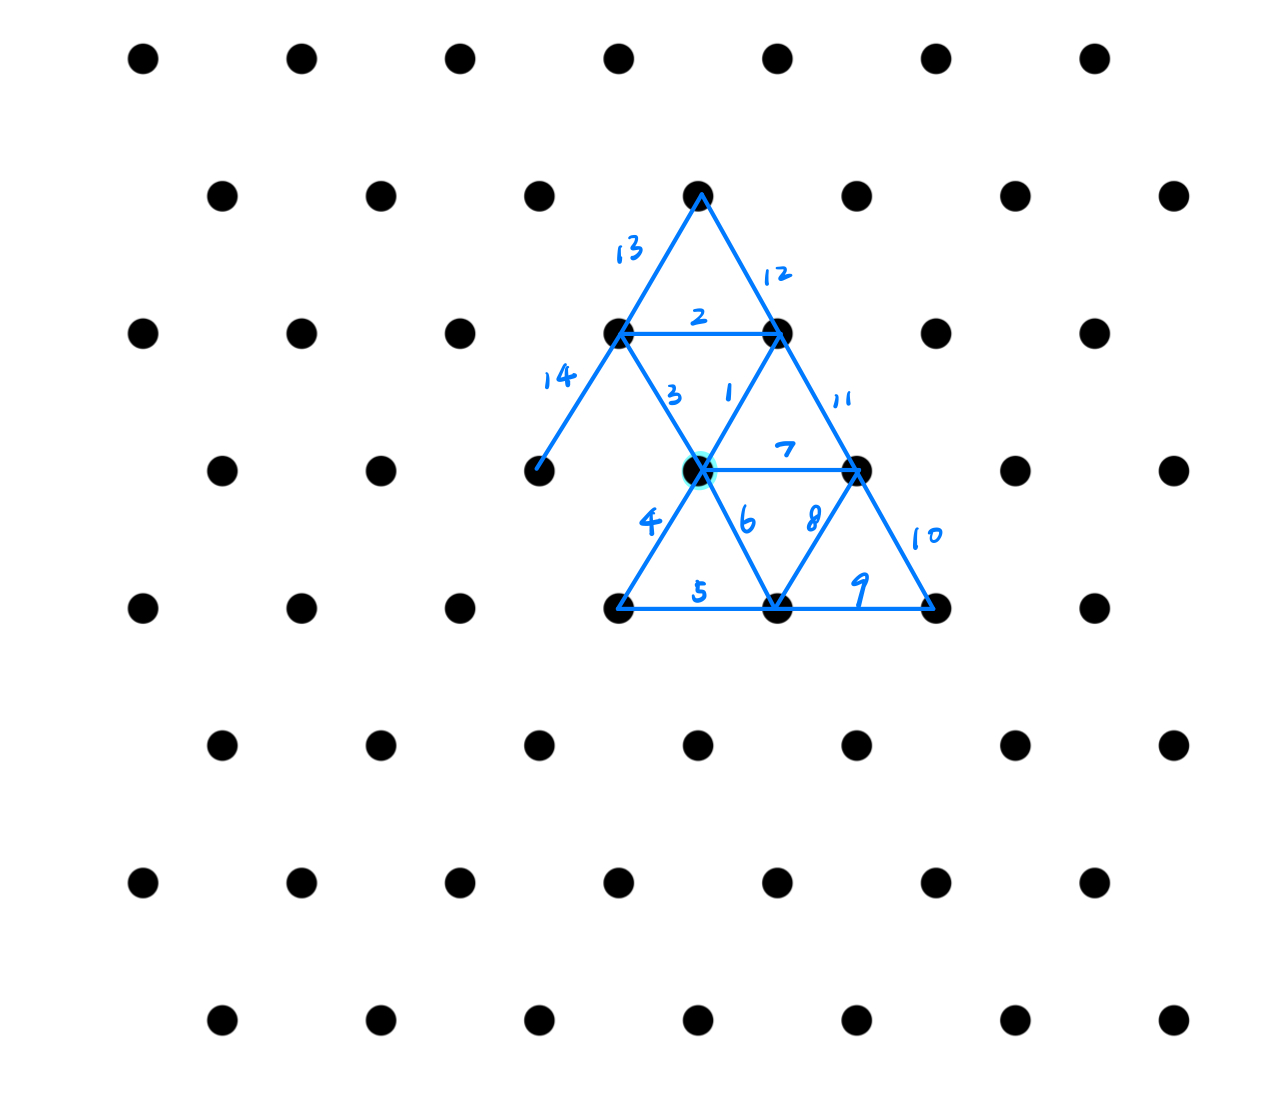
\includegraphics[width=\textwidth]{figure/fig6.png}}
			
				\centerline{Step 1}
			\end{minipage}
			\begin{minipage}{0.32\linewidth}
				\vspace{3pt}
				\centerline{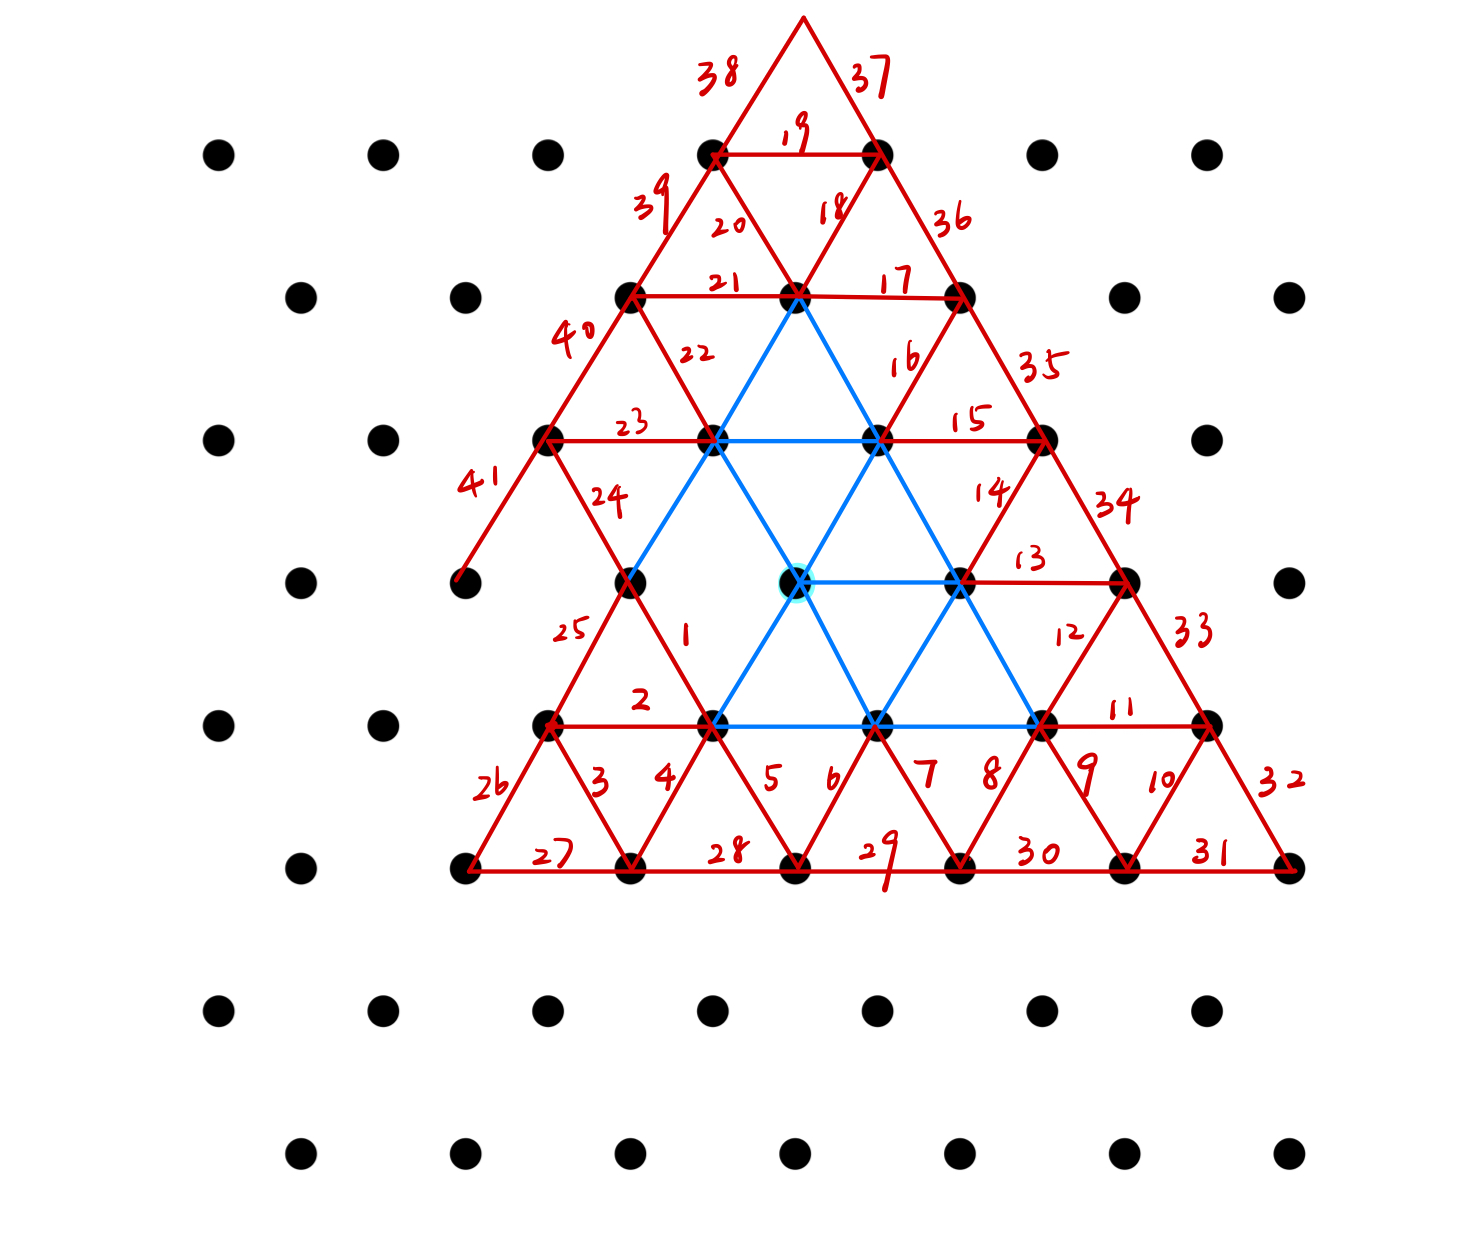
\includegraphics[width=\textwidth]{figure/fig7.png}}
			 
				\centerline{Step 2}
			\end{minipage}
			\begin{minipage}{0.32\linewidth}
				\vspace{3pt}
				\centerline{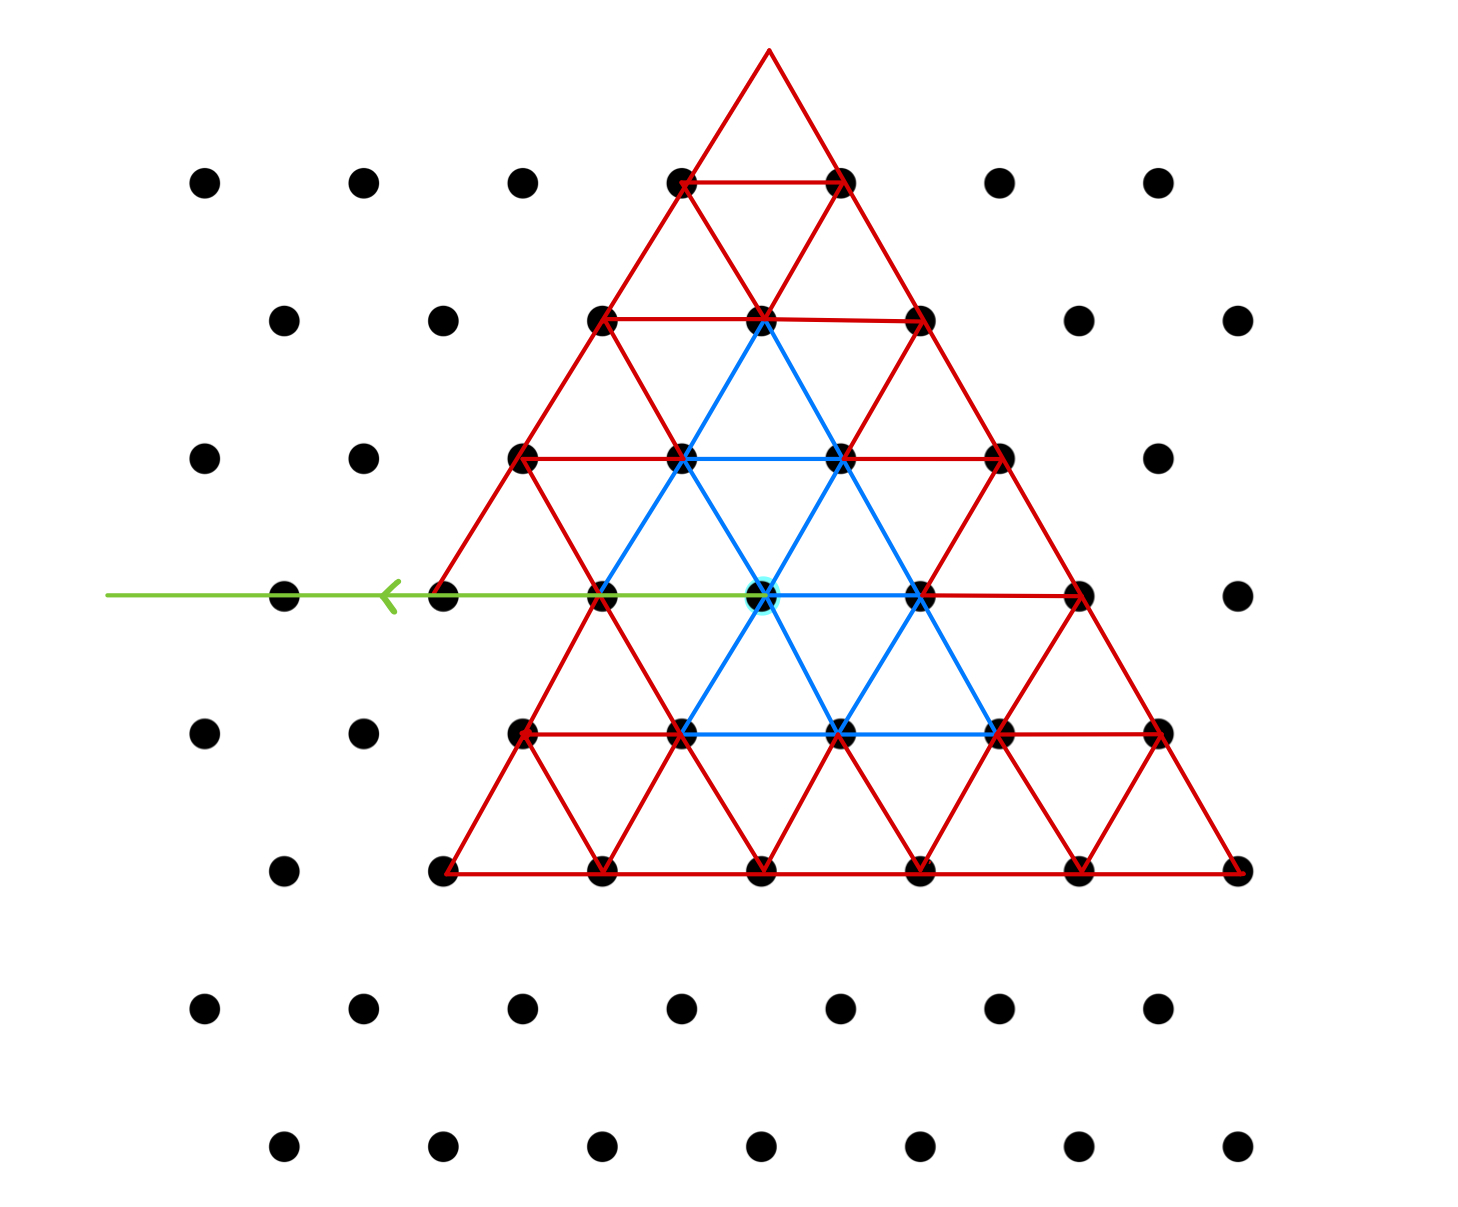
\includegraphics[width=\textwidth]{figure/fig8.png}}
			 
				\centerline{Step 3}
			\end{minipage}
			\caption{Construction of Euler trail}
			\label{fig:Construction}
		\end{figure}
		As shown in Fig \ref{fig:Construction}, there is a two-way infinite trail that includes every
		edge of $S$, where the green one is one trail, and the other can be extended to an infinite trail in the 
		same way as the figure. 

			\item We have shown that $S$ is Eulerian, then it suffices to show that $S$ is a countable connected graph.
			
			Since $S$ is Eulerian, each two vertices can be connected by a path. Thus $S$ is a connected locally countable infinite graph
			since ever vertex in $S$ has degree $6$. Apply Theorem $1.4$, $S$ is a countable graph, the result follows.
		\end{enumerate}
		
		
		
	\end{solution}

	\begin{problem}
		(Exercise 2.29(v))

		For which values of $k$ is the $k$-cube $Q_k$ Hamiltonian?
	\end{problem}

	\begin{solution}
		We show $Q_k$  is Hamiltonian for all $k\geq 2$ by induction. 
		
		For $k= 0,1$, there is no Hamiltonian cycle. For $k = 2$, $Q_2$ actually is $C_4$, which is a Hamiltonian cycle, so the statement is true for $n = 2$.

		Now, suppose $Q_k$ has a Hamiltonian circuit $C$. We can construct $Q_{k+1}$ from taking two copies of $Q_k$, then adding 0 to the end of the vertex bit-strings in one copy of $Q_k$, and adding 1 in the other.
		Take $k = 2$ as an example in Figure \ref{fig:Q}.

		\begin{figure}[H]
			\small
			\centering
			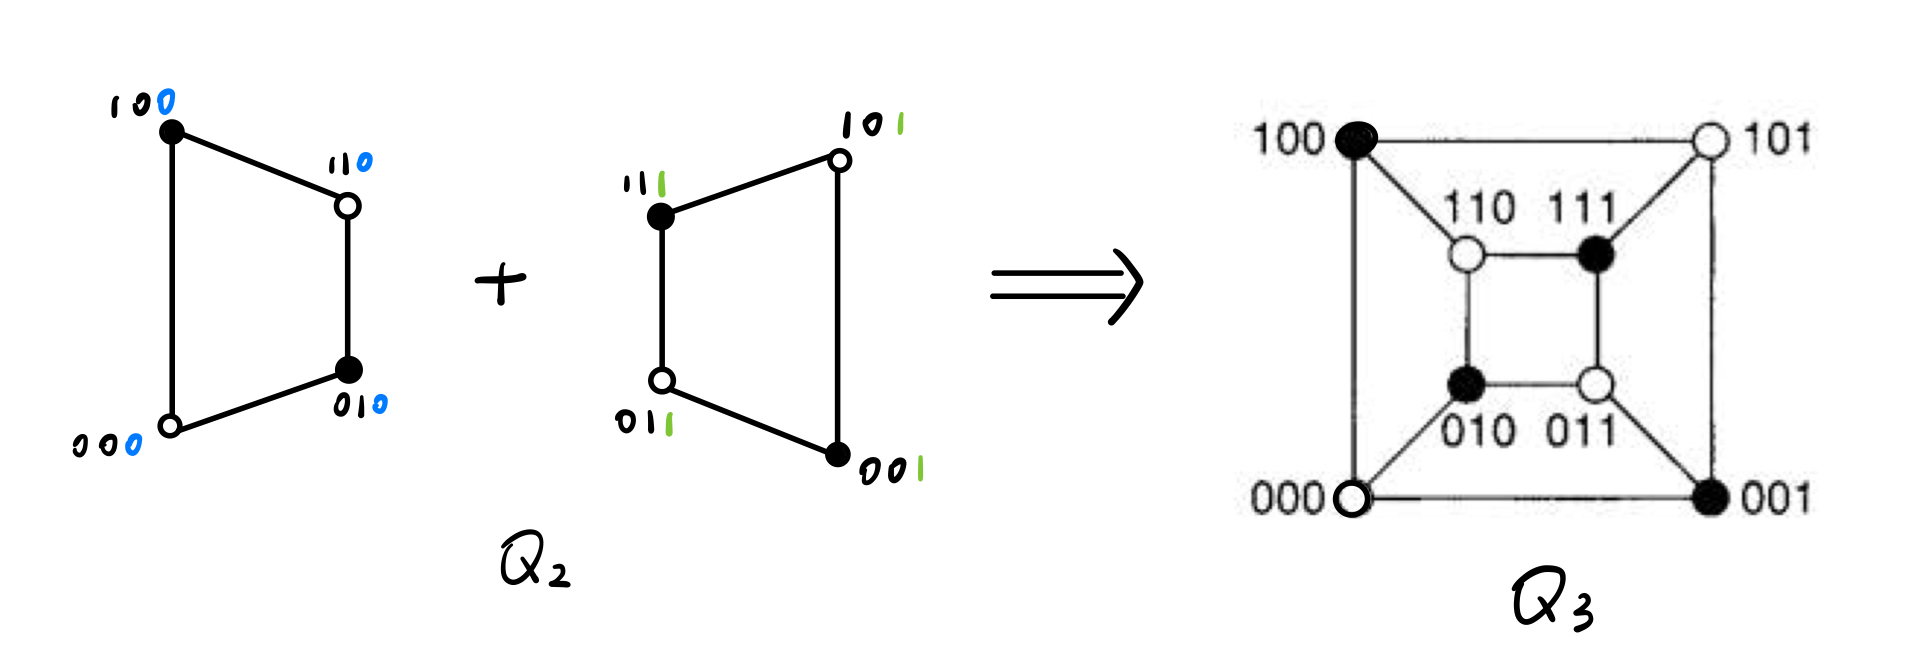
\includegraphics[width=0.75\columnwidth]{figure/fig9.png}
			\caption{Example}
			\label{fig:Q}
		\end{figure}
		In the first copy, take the Hamiltonian cycle $C$, and delete the final edge to form a Hamiltonian path $H$ and label the start and end vertices $v_1$ and $v_2$ respectively. 
		Then, join $v_2$ to $w_2$, the corresponding vertex in the second copy of $Q_k$, and reverse the path $H$ to get another Hamiltonian path in the second copy of $Q_k$ that ends at $w_1$. 
		As $w_1$ is adjacent to $v_1$, join these two vertices with a final edge that thus completes the Hamiltonian cycle. Hence, $Q_{k+1}$ has a Hamiltonian cycle whenever $Q_k$ does, so by induction $Q_k$ has a Hamiltonian circuit for all $k \geq 2$.

	\end{solution}


	\begin{problem}
		(Exercise 2.34)

		\begin{enumerate}
			\item[(i)] Let \( G \) be a graph with \( n \) vertices and \( \frac{1}{2}(n-1)(n-2) + 2 \) edges. Use Ore's theorem to prove that \( G \) is Hamiltonian.
			\item[(ii)] Find a non-Hamiltonian graph with \( n \) vertices and \( \frac{1}{2}(n-1)(n-2) + 1 \) edges.
		\end{enumerate}
		
	\end{problem}

	\begin{solution}
		\begin{enumerate}[(i)]
			\item Let $G$ be a simple graph with $n$ vertices and $m = \frac{1}{2}(n - 1)(n - 2) + 2$ edges. Let $u$, $v$ be two non-adjacent vertices of $G$, and let $v_1, \ldots, v_{n-2}$ be the other $n-2$ vertices of $G$.

	Consider the subgraph $H$ of $G$ induced by the vertices $v_1, \ldots, v_{n-2}$. This is the subgraph containing all edges of $G$ with both endpoints from the set $\{v_1, \ldots, v_{n-2}\}$.

	Since the number of edges in $H$ is at most $\binom{n-2}{2} = \frac{1}{2}(n - 2)(n - 3)$, there are at least
	\[
		\frac{1}{2}(n - 1)(n - 2) - \frac{1}{2}(n - 2)(n - 3) + 2 = n
	\]
	edges in $G$, each with exactly one endpoint $u$ or $v$ (since $u, v$ are not adjacent). In other words, $\text{deg}(u) + \text{deg}(v) \geq n$. Ore's theorem now proves $G$ is hamiltonian.
	
			\item The required non-Hamiltonian graph is constructed by taking a complete graph $K_{n-1}$
			  and adding a new vertex connected by a single edge to one of the vertices in $K_{n-1}$.

			  we obtain a graph with \( \frac{1}{2}(n-1)(n-2) + 1 \)edges. This new vertex has degree $1$, making it impossible to form a Hamiltonian cycle because a Hamiltonian cycle would require entering and exiting this vertex, which is not possible with only one edge.
			 
		\end{enumerate}
		

	\end{solution}

	\begin{problem}
		(Exercise 2.53) 

		Let \( G \) be a Hamiltonian graph and let \( S \) be any set of \( k \) vertices in \( G \). Prove that the graph \( G - S \) has at most \( k \) components.


	\end{problem}

	\begin{solution}
		Let $C$ be a Hamilton cycle in $G$. Fix any subset $S$ of $V$.

		We delete the vertices of $S$ from $C$. After the first vertex is deleted, $C$ is still connected, 
		but has become a path. When any of the subsequent $k - 1$ vertices is deleted, it either breaks some path into two shorter paths, 
		increasing the number of connected components by one or removes a vertex at an end of some path, leaving the number of connected components unchanged, or reducing it by one if this component was a $N_0$. 
		So $C \setminus S$ has at most $1 + (k - 1) = k$ connected components.

		Notice that if two vertices $u$ and $v$ are in the same connected component of $C \setminus S$, then they will also be in the same connected component of $G \setminus S$. 
		This is because adding edges can only connect things more fully, reducing the number of connected components. For example, if there is a $u - v$ walk in $C$, 
		then any pair of consecutive vertices in that walk is adjacent in $C$ so is also adjacent in $G$. Therefore the same walk is a $u - v$ walk in $G$. This tells us that the number of connected components of $G \setminus S$ is at most the number of connected components of $C \setminus S$, which we have shown to be at most $k$.

	\end{solution}
\end{document}


